% ---	
% primeiro capitulo de Resultados
% ---
\chapter{Modelos de \textit{Machine Learning}}


Além das funcionalidades descrita na função anterior, o objetivo da aplicação propõe um estudo mais aprofundado sobre características dos usuários que estão disseminando o conteúdo minerado. Utilizando algoritmos de redes complexas (como o grafo direcionado que descreve as interações entre os usuários da base) e de aprendizado de máquina, é possível classificar esses usuários por aspectos que não são tão triviais de identificar através de uma simples inspeção. No contexto da aplicação, dois aspectos foram levados em consideração para fazer essa classificação: a identificação de usuários influentes na rede e quais são os potenciais perfis \textit{fakes} (falsos). Todo o processo proposto pelo modelo pode ser visualizado no \textit{canvas}\footnote{\href{https://towardsdatascience.com/a-data-science-workflow-canvas-to-kickstart-your-projects-db62556be4d0}{https://towardsdatascience.com/a-data-science-workflow-canvas-to-kickstart-your-projects-db62556be4d0}} da figura \ref{fig:canvas}.

\begin{figure}[!htb]
\centering
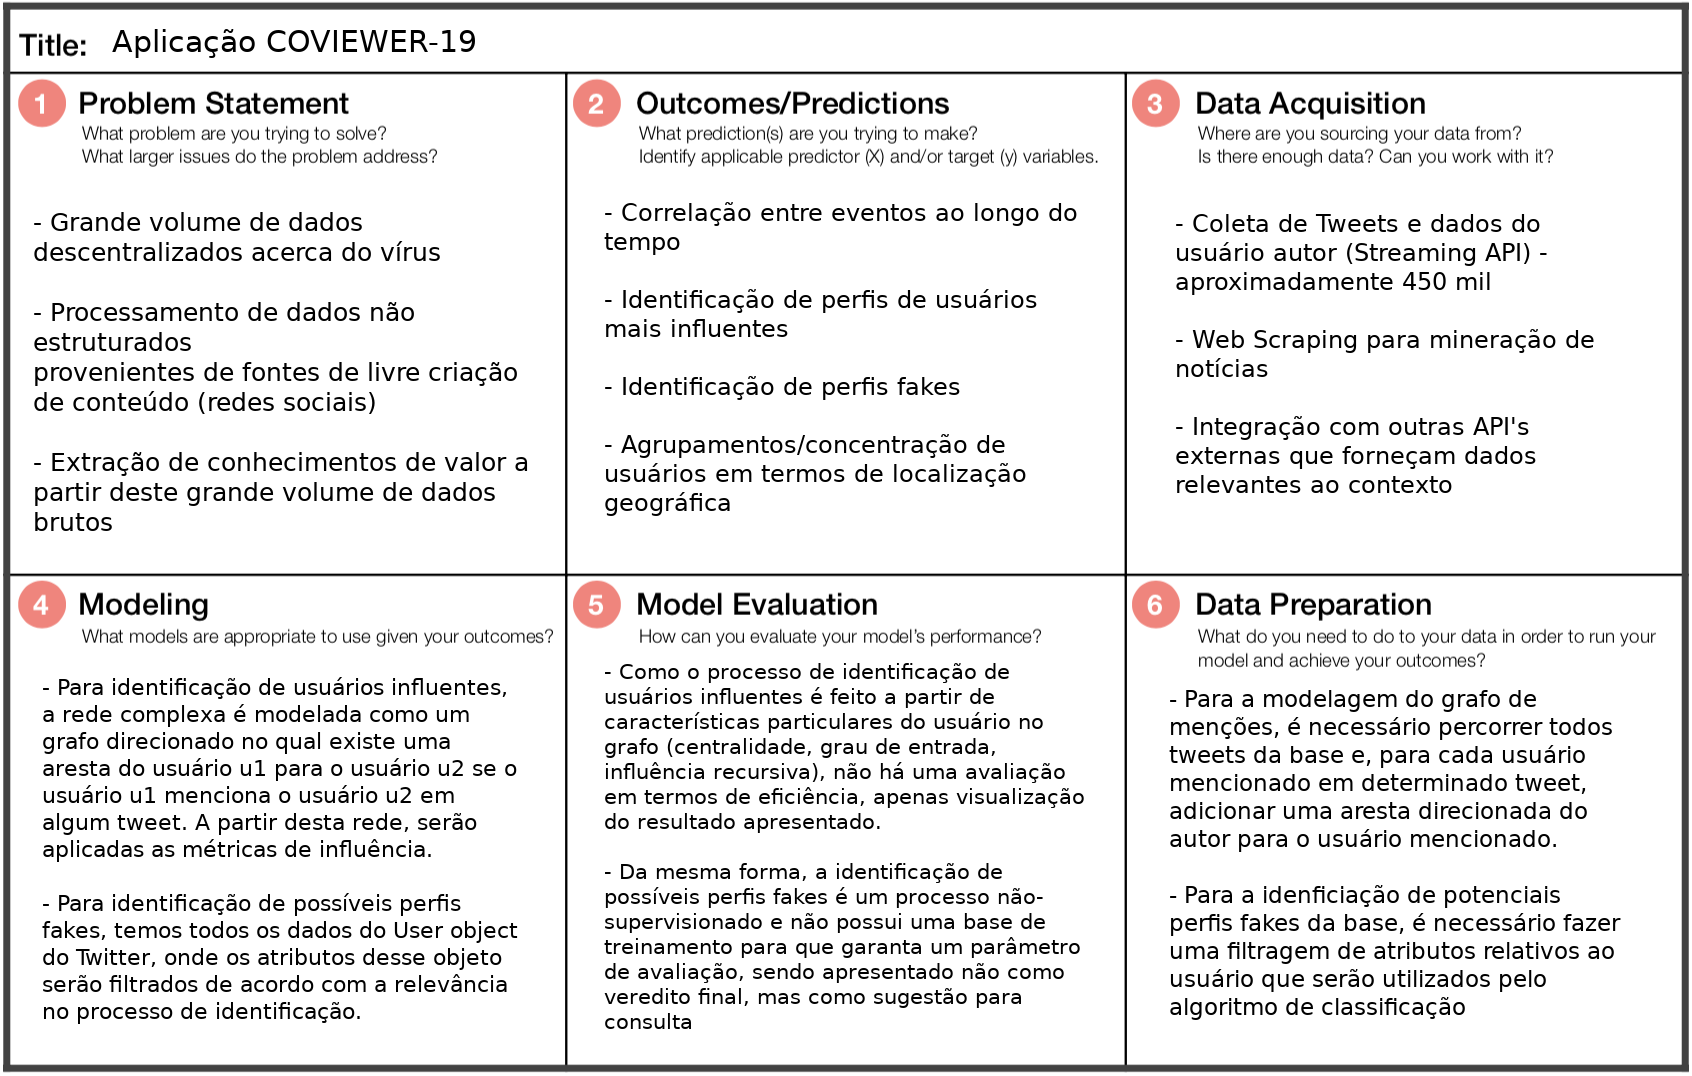
\includegraphics[width=16cm]{img/20.png}
\caption[Caption for LOF]{ \textit{Canvas} do modelo de aprendizado de máquina proposto }
\label{fig:canvas}
\end{figure}


\section{Identificação de Usuários Influentes}

A princípio, a noção trivial de um usuário influente em uma rede complexa que descreve qualquer rede social seria o número de seguidores desse usuário. Mas uma análise mais apurada pode revelar a medida de influência sob diferentes perspectivas, considerando-se principalmente o fato de que o número absoluto de seguidores não reflete necessariamente o engajamento. Na aplicação proposta, além de exibir os usuário mais influentes pelo número absoluto de seguidores, analisa-se também a medida de influência a partir de outras 3 métricas: o grau de entrada, o \textit{pagerank}\footnote{\href{https://www.prime4web.com.br/google-pagerank}{https://www.prime4web.com.br/google-pagerank}} e o \textit{betweeness}\footnote{\href{https://homepages.dcc.ufmg.br/~valdete/metricas/aula\_metricas\_grafos.pdf}{https://homepages.dcc.ufmg.br/~valdete/metricas/aula\_metricas\_grafos.pdf}}. 
	
Enquanto o número de absoluto de seguidores pode ser diretamente filtrado através de um \textit{sort} no atributo correspondente na base, as demais métricas requerem uma modelagem em um grafo direcionado G = (V, E), de forma que, cada elemento de V representa um usuário que gera tweets ou é mencionado em um \textit{tweet}, e o conjunto E é composto por arestas que indicam uma relação entre um par de usuários, na qual existe uma aresta direcionada do usuário u\textsubscript{1} para o usuário u\textsubscript{2} se o usuário u\textsubscript{1} mencionou o usuário u\textsubscript{2} em algum \textit{tweet}. 

A partir desta rede de menções obtida, a métrica de grau de entrada implica, trivialmente, no usuário que foi mais mencionado na base. O \textit{pagerank}, por sua vez, leva em consideração não só uma medida quantitativa mas também qualitativa das arestas que apontam para um usuário. Em um exemplo básico, se um usuário u\textsubscript{1} tem poucas arestas incidindo sobre ele, mas uma delas é de um usuário u\textsubscript{2} muito influente na rede, o conteúdo disseminado pelo usuário u\textsubscript{1} ganha uma maior relevância em termos de influência. Por fim, o \textit{betweenness} é uma medida de centralidade na rede, que indica uma medida de intermediação do vértice em caminhos mais curtos.

Esse formato permite utilizar as funções pré-implementadas da biblioteca \textit{igraph}\footnote{\href{https://igraph.org/python/}{https://igraph.org/python/}} (em \textit{python}), à partir do uso de sua estrutura, que foi implementada como descreve a figura \ref{fig:redeigraph}. Os valores para os retornos de \textit{pagerank} e \textit{betweenness} foram normalizados de forma a indicar os valores da medida entre 0 e 1, sendo 1 a medida mais alta obtida na base. Para o grau de entrada, por se tratar de uma contagem, optou-se por apresentar em números absolutos.

\begin{figure}[!htb]
\centering
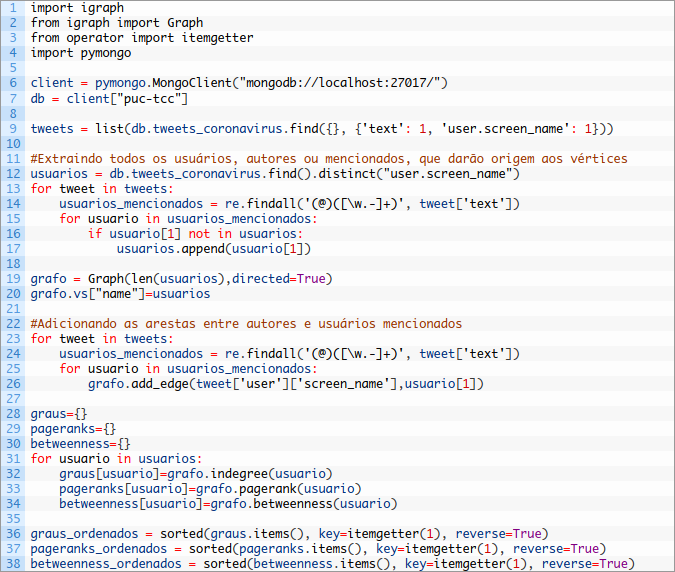
\includegraphics[width=15cm]{img/21.png}
\caption{ Montando a rede de menções no \textit{igraph} para classificação de usuários influentes pelas métricas }
\label{fig:redeigraph}
\end{figure}

De forma similar às demais funcionalidades que não alteram sua resposta na base já coletada, o \textit{endpoint} da aplicação teve seu retorno cacheado. Especialmente neste caso, a aplicação das métricas à rede demandam muito recurso em termos de tempo de processamento e memória (a biblioteca \textit{igraph} utiliza uma matriz de adjacência como estrutura de dados, o que implica em um consumo de memória de crescimento quadrático de acordo com o número de usuários). Dessa forma, apesar do longo tempo de processamento para obtenção dos resultados na primeira chamada, as subsequentes já contam com a resposta em \textit{cache}. Uma visão geral da apresentação desses usuários na \textit{view} é apresentada na figura \ref{fig:usuariosinfluentes}.

\begin{figure}[!htb]
\centering
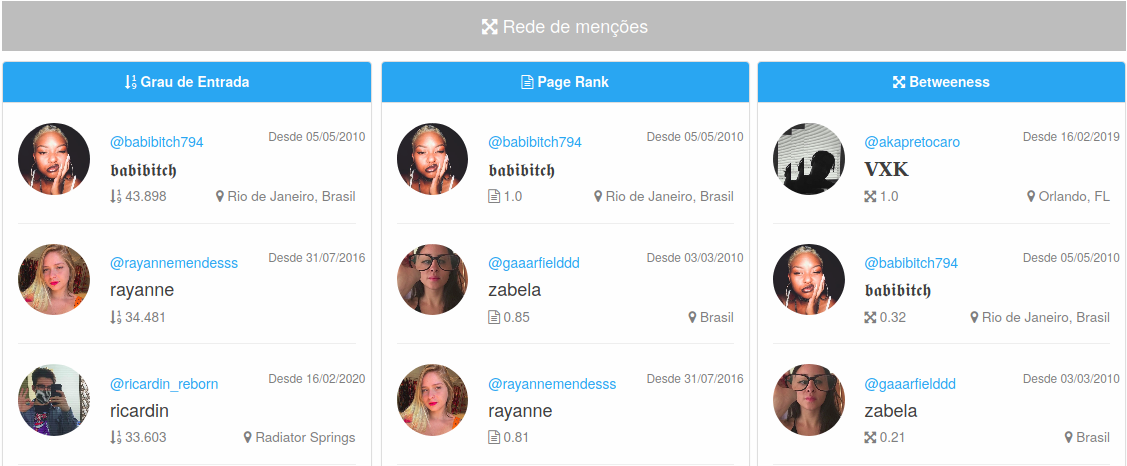
\includegraphics[width=15cm]{img/22.png}
\caption{ Visão geral da funcionalidade de usuários influentes da base }
\label{fig:usuariosinfluentes}
\end{figure}

\section{Identificação de Potenciais Perfis Falsos}
	Para a identificação de usuários com perfis \textit{fakes} (que não remetem a um perfil pessoal, podendo ser operado de forma automática - \textit{bots} - ou não, e que consequentemente comprometem a confiabilidade do conteúdo), optou-se por um algoritmo de classificação não-supervisionado. Na ausência de uma base pública disponível similar (pré-classificada por supervisão humana), a estratégia para implementação de forma não-supervisionada foi motivada pela proposta do BigDataProject3\footnote{\href{https://github.com/lnyaki/BigDataProject3}{https://github.com/lnyaki/BigDataProject3}} para detecção automática de perfis falsos.
	
	Esse conjunto de diretrizes enumerados nas figuras \ref{fig:camizani} e \ref{fig:crescia} propõe um método de avaliação automática para cada usuário, baseado em verificações pontuais que incrementam ou decrementam um \textit{score} desse perfil de acordo com características que indicam a autenticidade de um perfil em rede social. Entretanto, algumas das diretrizes não podem ser verificadas na base da aplicação pois se referem a características mais complexas que envolvem a análise de publicações do usuário (minerar essas informações para uma base tão grande seria inviável devido à limitação de requisições da API). Além disso, foram utilizados pesos de acordo com a relevância da diretriz: O conjunto híbrido das diretrizes observáveis utilizadas que determina o \textit{score} (inicialmente zerado) é descrito na lista que segue.


\begin{itemize}
	\item Nome presente: +1 
	\item Imagem de perfil presente: +1 
	\item Localidade presente: +1 
	\item Descrição (bio) presente: +1 
	\item Número de seguidores > 100: +1 
	\item Presente na lista de pelo menos algum outro usuário: +1 
	\item Tem pelo menos 100 \textit{posts}: +1 
	\item URL (\textit{website}) presente: +1 
	\item Utiliza Twitter Web, Android ou iOS: +1 
	\item O número de seguidores é pelo menos o dobro de quem está seguindo: +1 
	\item A conta existe há pelo menos 5 anos: +1 
	\item A descrição (bio) contém o termo "bot": -1 
	\item A quantidade de números no \textit{screen\_name} é maior do que 5: -1 
	\item O número de seguidores é 50 vezes menor do que está seguindo: -3

\end{itemize}	

\begin{figure}[!htb]
\centering
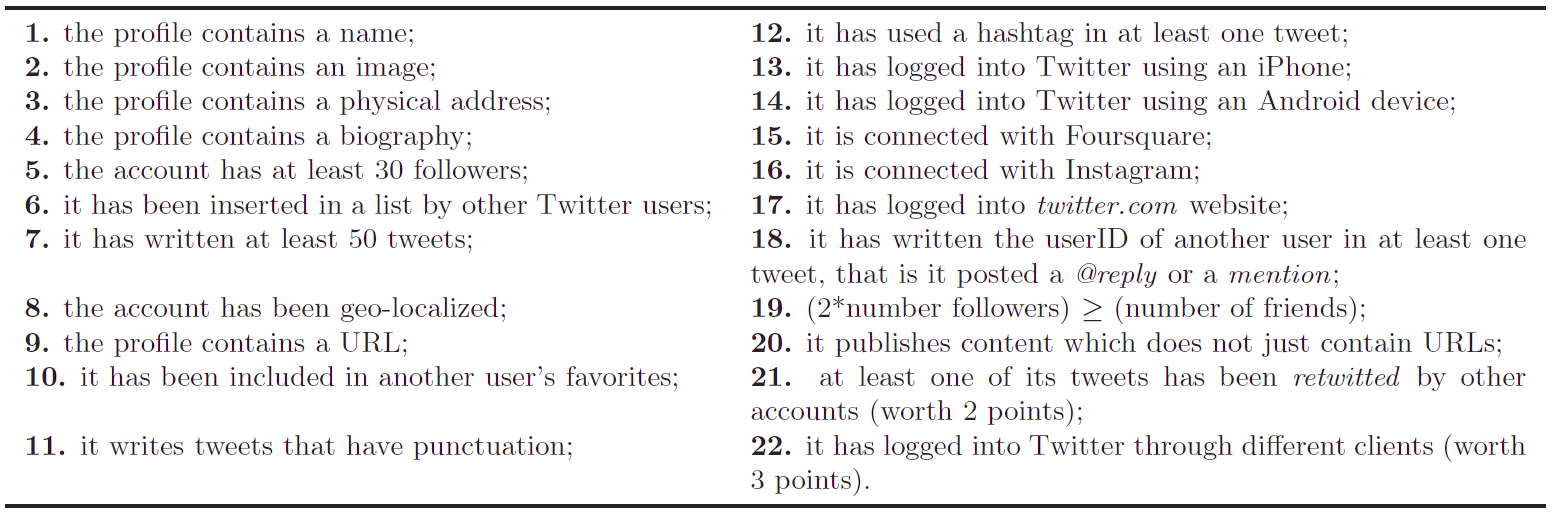
\includegraphics[width=15cm]{img/23.png}
\caption[Caption for LOF]{ Diretrizes propostas por Camizani-Calzolari\footnotemark}
\label{fig:camizani}
\end{figure}

\footnotetext{\href{https://blog.ida.cl/wp-content/uploads/sites/5/2014/07/Twitter-study.pdf}{https://blog.ida.cl/wp-content/uploads/sites/5/2014/07/Twitter-study.pdf}}


\begin{figure}[!htb]
\centering
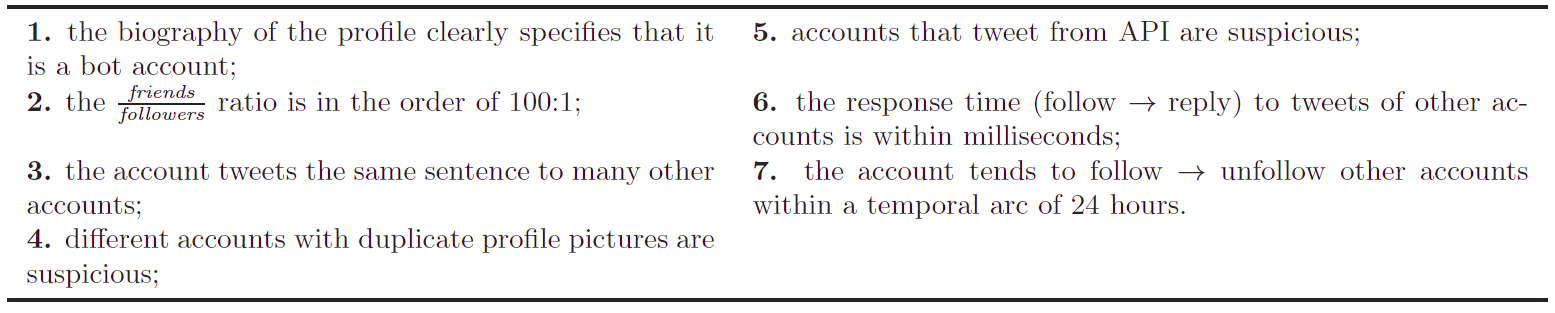
\includegraphics[width=15cm]{img/24.png}
\caption[Caption for LOF]{ Diretrizes propostas por (CRESCIA et al, 2015)\footnotemark}
\label{fig:crescia}
\end{figure}

\footnotetext{\href{https://core.ac.uk/download/pdf/37831629.pdf}{https://core.ac.uk/download/pdf/37831629.pdf}}

	Para fazer essa contabilização e definir uma nova coluna \textit{verify\_score} (uma vez que esse valor não se altera) que será consultada posteriormente, a classe MongoHelper implementou o método descrito
na figura \ref{fig:metodoscore}
	
	
\begin{figure}[!htb]
\centering
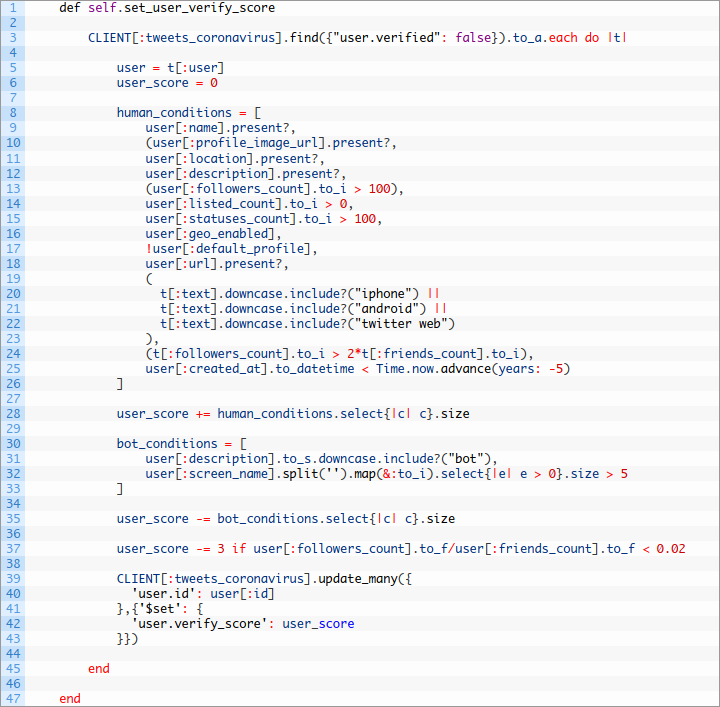
\includegraphics[width=15cm]{img/25.png}
\caption[Caption for LOF]{ Método para contabilização dos \textit{scores} dos usuários da base}
\label{fig:metodoscore}
\end{figure}
	
	
	Obtendo-se esse \textit{score} para todos os usuários da base, a funcionalidade fundamentalmente consiste na listagem desses potenciais usuários de acordo com o valor de \textit{score} que atua como limiar. Empiricamente, através de observação na própria base, esse valor foi aproximado para um \textit{score} menor ou igual a 2. Como a listagem desses usuários é feita em uma \textit{datatable} (de forma muito similar à listagem de todos os \textit{tweets}), um método também similar para listagem, paginação e busca foi implementado no MongoHelper. Alguns registros de exemplo podem ser visualizados na figura \ref{fig:fakeusers}.
	
\begin{figure}[!htb]
\centering
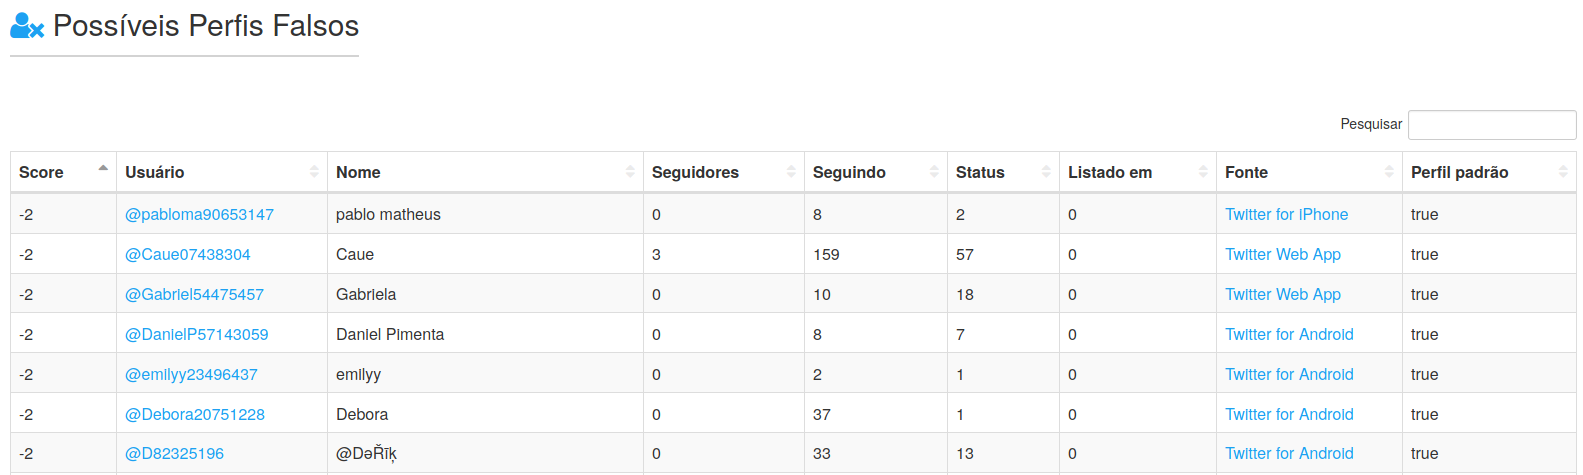
\includegraphics[width=15cm]{img/27.png}
\caption[Caption for LOF]{ Listagem de alguns do potenciais perfis falsos na \textit{datatable}}
\label{fig:fakeusers}
\end{figure}
	
